%  figure placement: here, top, bottom, or page
\begin{figure}
   \centering
   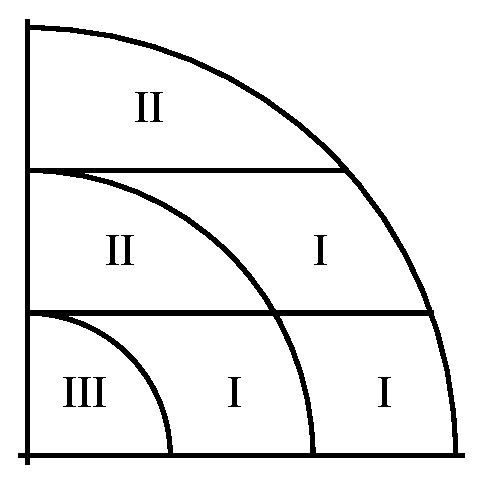
\includegraphics[ width = 1in ]{graphics/integrals.eps}  \\
   \caption{Area of the upmost limb computed using geometrical methods. The result is shown in \eqref{eq:area I} and \eqref{eq:area II}.}
   \label{fig:sector integrals}
\end{figure}

\endinput  %  .  .  .  .  .  .  .  .  .  .  .  .  .  .  .  .  .  .